% Created 2021-11-17 Wed 11:20
% Intended LaTeX compiler: pdflatex
\documentclass[14pt]{beamer}\usepackage{listings}
\usepackage{color}
\usepackage{amsmath}
\usepackage{array}
\usepackage[T1]{fontenc}
\usepackage{natbib}
\lstset{
keywordstyle=\color{blue},
commentstyle=\color{red},stringstyle=\color[rgb]{0,.5,0},
literate={~}{$\sim$}{1},
basicstyle=\ttfamily\small,
columns=fullflexible,
breaklines=true,
breakatwhitespace=false,
numbers=left,
numberstyle=\ttfamily\tiny\color{gray},
stepnumber=1,
numbersep=10pt,
backgroundcolor=\color{white},
tabsize=4,
keepspaces=true,
showspaces=false,
showstringspaces=false,
xleftmargin=.23in,
frame=single,
basewidth={0.5em,0.4em},
}
\usepackage{natbib, dsfont, pgfpages, tikz,amssymb, amsmath,xcolor}
\bibliographystyle{abbrvnat}
\usepackage{enumerate}
% New operators and commands
\newcommand{\Z}{\mathbb{Z}}
\newcommand{\Q}{\mathbb{Q}}
\newcommand{\R}{\mathbb{R}}
\newcommand{\N}{\mathbb{N}}
\newcommand{\C}{\mathbb{C}}
\renewcommand{\S}{\mathbb{S}}
\newcommand{\blank}{\makebox[1ex]{\textbf{$\cdot$}}}
\newcommand\independent{\protect\mathpalette{\protect\independenT}{\perp}}
\def\independenT#1#2{\mathrel{\rlap{$#1#2$}\mkern2mu{#1#2}}}
\renewcommand{\phi}{\varphi}
\renewcommand{\epsilon}{\varepsilon}
\newcommand*\diff{\mathop{}\!\mathrm{d}}
\newcommand{\weakly}{\rightsquigarrow}
\newcommand\smallO{
  \mathchoice
    {{\scriptstyle\mathcal{O}}}% \displaystyle
    {{\scriptstyle\mathcal{O}}}% \textstyle
    {{\scriptscriptstyle\mathcal{O}}}% \scriptstyle
    {\scalebox{.6}{$\scriptscriptstyle\mathcal{O}$}}%\scriptscriptstyle
}
\newcommand{\midd}{\; \middle|\;}
\newcommand{\1}{\mathds{1}}
\usepackage{ifthen} %% Empirical process with default argument
% \newcommand{\G}[1][]{%
%    \ifthenelse{ \equal{#1}{} }
%       {\ensuremath{\mathbb{G}_n}}
%       {\ensuremath{\mathbb{G}_{#1}}}
% }
% New version:
\newcommand{\G}[2][n]{
{\ensuremath{\mathbb{G}_{#1}}{\left[#2\right]}}
}
\DeclareMathOperator*{\argmin}{\arg\!\min}

% New operators for consistent notation
\newcommand{\V}{\mathrm{Var}} % variance
\newcommand{\measure}[1]{\mathrm{{#1}}} % measure
% \newcommand{\measure}[1]{\textnormal{\textbf{{#1}}}} % measure
\newcommand{\m}[1]{\measure{#1}} % measure shortcut
\newcommand{\eqd}{\stackrel{d}{=}} % equality in distribution
\newcommand{\arrow}[1]{\xrightarrow{\; {#1} \;}}
\newcommand{\arrowP}{\xrightarrow{\; \m{P} \;}} % convergence in probability
\newcommand{\leb}{\lambda} % the Lebesgue measure
\newcommand{\T}{\top} % transpose
\newcommand{\KL}{\ensuremath{D_{\mathrm{KL}}}}

\usepackage{xargs}
% Make it easy to change counterfactual notation:
\newcommandx{\cf}[4][3={}, 4={}]{
  % \ifthenelse{ \equal{#4}{} }
  % {{#1^{#2}}(#3)}
  {\ifthenelse{ \equal{#3}{} }
    {{#1^{#2}}_{#4}}
    {{#1^{#2}}_{#4}(#3)}}
}

% Easily change notation:
\DeclareMathOperator{\TT}{\Psi} % target parameter
\newcommand{\lp}{\mathcal{L}_{\P}^2} % shortcut for lp2 space
\newcommand{\empmeas}{\hat{\mathbb{P}}_n} % empirical measure
\DeclareMathOperator{\E}{\mathbb{E}} % expectation
\renewcommand{\P}{\m{P}} % probability
\newcommand{\ic}{\mathrm{IF}} % influence curve
\usecolortheme{crane}
\beamertemplatenavigationsymbolsempty
\setbeamercolor{gray}{bg=white!90!black}
\setbeamertemplate{itemize items}{$\circ$}

\renewcommand*\familydefault{\sfdefault}
\itemsep2pt
\usepackage[utf8]{inputenc}
\usepackage[T1]{fontenc}
\usepackage{graphicx}
\usepackage{grffile}
\usepackage{longtable}
\usepackage{wrapfig}
\usepackage{rotating}
\usepackage[normalem]{ulem}
\usepackage{amsmath}
\usepackage{textcomp}
\usepackage{amssymb}
\usepackage{capt-of}
\usepackage{hyperref}
\usetheme{default}
\date{November 17, 2021}
\title{Young statistical research in Denmark}
\titlegraphic{
\includegraphics[height=3cm]{logo.png}}
\begin{document}

\maketitle
\logo{
\includegraphics[height=1.5cm]{logo.png}}

\section{Intro}
\label{sec:org03ba68e}
\begin{frame}[label={sec:org13d5759}]{Young Statisticians Denmark (YSD)}
\small

A society that plans social and scientific events, especially for students and young
professionals working with statistics.
\vfill

\begin{itemize}
\item Share knowledge in a relaxed atmosphere.
\item ``Young'' and ``Statistician'' is broadly defined.
\item Part of the Danish Society for Theoretical Statistics.
\end{itemize}

\vfill     
\end{frame}

\begin{frame}[label={sec:orgf8a4dd2}]{Previous events}
22 events since 2015.

\vfill

\begin{center}
\begin{tabular}{l}
\emph{Neurobiology meets Statistics}\\
\emph{Science talk and pub quiz}\\
\emph{Career event}\\
\emph{Talking about the p-word}\\
\ldots{}\\
\end{tabular}

\end{center}
\end{frame}

\begin{frame}[label={sec:orgfe98e3b}]{Crowd}
\begin{center}
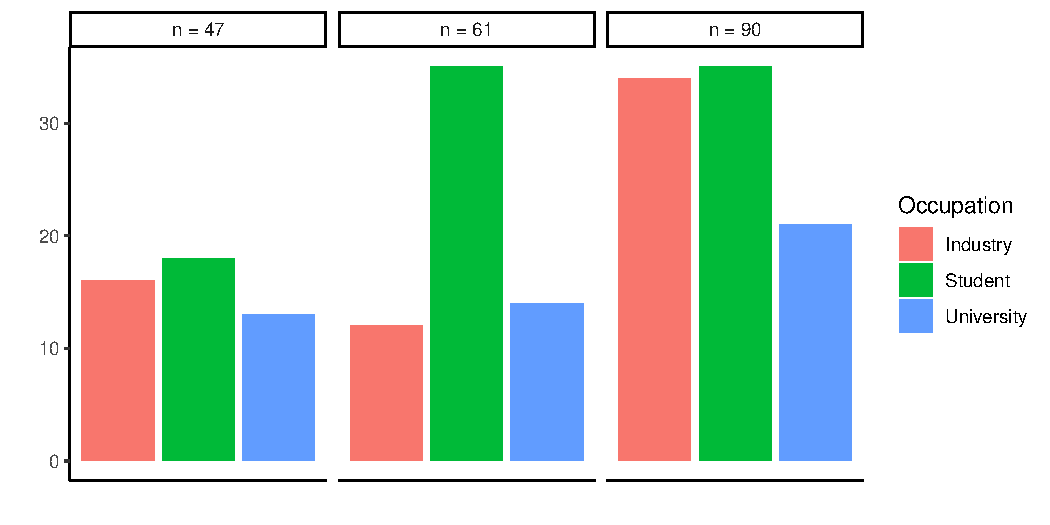
\includegraphics[width=.9\linewidth]{./crowd-plot.pdf}
\end{center}
\end{frame}

\begin{frame}[label={sec:org2020877}]{Upcoming events}
2 upcoming events within the next two months.

\vfill

\begin{description}
\item[{November 23}] Statisticians in the wild (vol. 2)
\item[{January 13}] Event on causality
\end{description}

\vfill
\end{frame}

\begin{frame}[label={sec:org838907e}]{Young statistical research in Denmark}
What questions occupy the minds of young statistical researchers in Denmark? What topics do they
spend their time on studying?
\end{frame}

\section{Sneha}
\label{sec:orgf26f6cb}
\begin{frame}[label={sec:org3654c08}]{YSD presents:}
\begin{block}{\centering Sneha Das}
\small
\begin{itemize}
\item Postdoc at the Section of Statistics and Data Analysis (The Technical University of Denmark)
\item PhD from Aalto University Finland (defense in one week)
\end{itemize}
\end{block}
\end{frame}
\begin{frame}[label={sec:orgb9e2213}]{}
\end{frame}
\section{Nikolaj}
\label{sec:org02c02e1}
\begin{frame}[label={sec:org77db46e}]{YSD presents:}
\begin{block}{\centering Nikolaj Thams}
\small
\begin{itemize}
\item PhD student at Copenhagen Causality Lab, MATH (University of Copenhagen)
\item Master in Statistics from University of Copenhagen
\end{itemize}
\end{block}
\end{frame}
\end{document}